%% Introduction: Length: 25-30 pages.
%%  * Relevant background, 
%%  * Outline of state of knowledge, 
%%  * emphasize outstanding questions 

\chapter{Introduction}
\label{ch:intro}

Given the constantly improving cost and speed of genome sequencing, it is reasonable to expect that within the coming decades personal genomes will be known for a substantial part of the global populace. Unfortunately, our limited ability to interpret the variation within stands in stark contrast with this development. Even when only considering mutations in coding regions of the genome, the effects of most missense variants are not known. While a number of computational approaches exist to make predictions as to the effects of coding variants, they are currently not reliable enough for clinical use. By comparison, laboratory assays produce more trustworthy results, but until recently did not scale to the space of all possible mutations. The development of Deep Mutational Scanning~\cite{fowler_high-resolution_2010} has now made this endeavour possible. In the following sections, each of these issues will be discussed in more detail.

\section{The Genotype-Phenotype Problem}
\label{introGenoPheno}

Linking genotype to phenotype is a very difficult problem. The part of the human genome we understand best are protein-coding genes, yet they only constitute a small fraction the whole. Impacts of mutations in other functional elements such as splice sites, promoters, or regulatory sequences are more difficult to assay, not to mention the vast stretches of intergenic space. While one might expect the latter to not bear functional significance \textit{a priori}, a large number of loci identified as correlated with diseases in genome-wide association studies (GWAS) are found within these regions~\cite{edwards_beyond_2013}. While many of these cases may simply be spurious findings due to linkage disequilibrium with variants in coding regions~\cite{tasan_selecting_2015}, more functions yet unknown may lie hidden within this vast space.  
But even for protein-coding sequences the problem is far from simple. Alleles with simple Mendelian behaviour are the exception rather than the rule. %TODO: REF?
Most phenotypes are complex, i.e. they emerge through the interplay of many different genetic or environmental factors. Conversely, many genes are also pleiotropic, i.e. they are involved more than one mechanism. As a result of this complexity, a mutation found in one person may not have the same effect as in another---a phenomenon called incomplete penetrance. Similarly, two different mutations within the same coding sequence will often not have the same effect either. Depending on how the translated protein is affected (e.g. catastrophic folding failure, alteration of a molecular interaction interface or active site, or a subtle change on an unused surface) the effects may differ in severity or in rare cases may even result in the emergence of new behaviours.

%Clinical perspective on the genotype-phenotype problem
Given the much greater difficulty of interpreting non-coding regions, %TODO: REF?
clinical applications have so far largely concentrated on protein-coding genes. Sequencing panels for known disease-associated genes and even whole-exome sequencing (WES) are widely commercially available. A number of different standards for classifying mutations with respect to their potential health impacts have been proposed. Most prominently, the American College of Medical Genetics and Genomics (ACMG) standard~\cite{richards_standards_2015}.
It defines categories stretching from ``pathogenic'' via ``variant of uncertain significance'' (VUS) to ``benign''. Even though the mutational landscape for a handful of genes, such as \gene{BRCA1} are explored better than others due to their established relevance and potential for taking clinical action~\cite{cheon_variants_2014}, the vast majority of clinical variants are currently classified as VUS. For example, in a recent study using gene panels assessing germline cancer risk loci~\cite{maxwell_evaluation_2016}, over 98\% of missense variants have been called VUS. Not only can these uncertainties burden patients with unnecessary anxiety~\cite{cheon_variants_2014}, they also call into question the value of sequencing in the clinic if the majority of findings are not actionable. With increasing use of WES over gene panels, this problem is only going to get worse. According to the 1000 Genomes Project data, every person carries 100-400 missense variants that are so rare that they have likely never been seen before in the clinic~\cite{the_1000_genomes_project_consortium_global_2015}. In the absence of previous observations they would automatically be added to the long list of VUS.

\section{\textit{In silico} approaches to variant function assessment}
\label{insilicoIntro}

A number of algorithms exist that offer predictions as to the deleteriousness of mutations, the most prominent ones being PolyPhen-2~\cite{adzhubei_predicting_2001}, SIFT~\cite{ng_predicting_2001} and PROVEAN~\cite{choi_predicting_2012}. PolyPhen-2 employs a machine learning method based on evolutionary conservation and protein structural features. It uses a set of previously reported pathogenic alleles as a positive training set and differences between human genes and their mammalian homologues as a negative training set. By contrast, SIFT (Sorting Intolerant From Tolerant) only uses evolutionary conservation. The tool uses multiple sequence alignments to calculate position-specific score matrices for each gene which are then normalized and transformed into probability values. PROVEAN (PROtein Variation Effect ANalyzer) similarly only takes into account sequence alignments. However, rather than just computing a position-specific score, PROVEAN calculates the difference in alignment quality between using the wildtype or variant sequence against clusters of homologous sequences. The average distance is then interpreted as indicative of the deleteriousness of the variant. 

While the three tools succeed in making good predictions, their reliability is unfortunately still not high enough to serve as a basis of clinical decision making. Song Sun and other members of the Roth Lab recently performed an independent comparison of these tools on a set of well established disease-causing variants as well as rare polymorphisms with no known disease association~\cite{sun_extended_2016}. A high precision (the fraction of correct classifications out of all positive classifications) can be considered especially important when considering taking clinical action based on a prediction. When compared at a minimum precision level of 90\%, PolyPhen-2 and PROVEAN only reach a sensitivity of 19\% and 21\%, respectively (where sensitivity is defined as the fraction of correct classifications out of all real existing disease variants). SIFT was not capable of achieving 90\% precision at any score threshold. In concordance with these limitations, the ACMG currently considers only cases in which multiple methodologically orthogonal prediction algorithms agree as weak evidence in a supporting role for VUS re-classification~\cite{richards_standards_2015}.

\begin{figure}[h!]
	\centering
	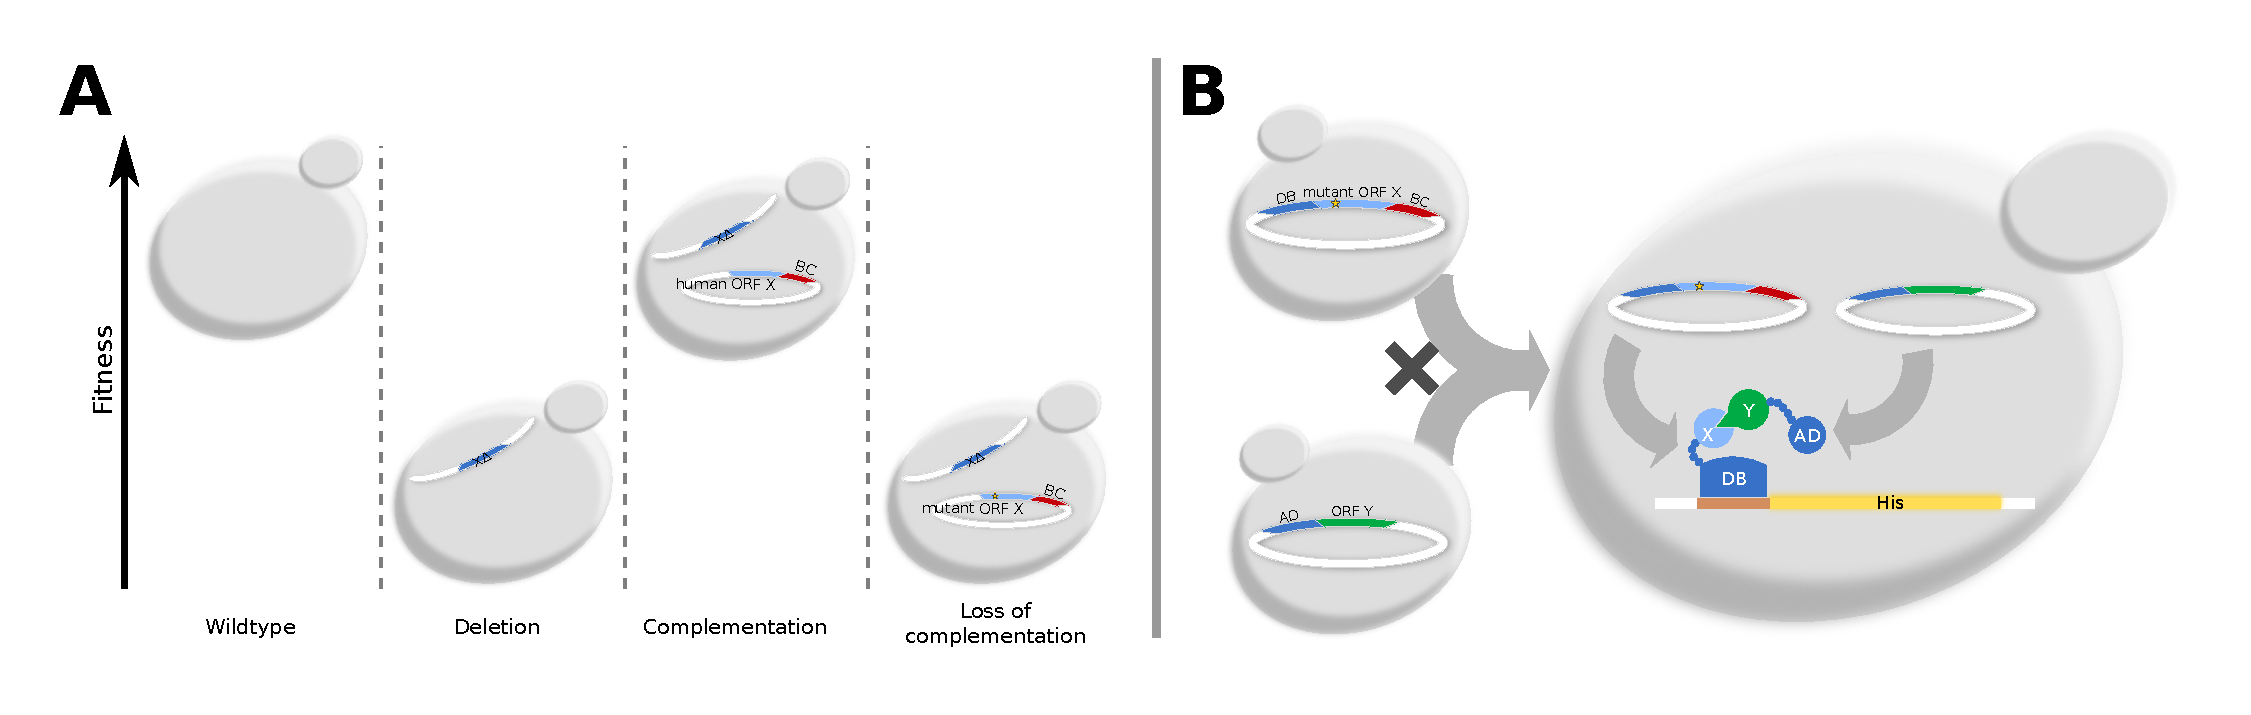
\includegraphics[width=\textwidth]{img/compl_y2h.pdf}
	\caption{Complementation and Yeast-2-Hybrid. A) Yeast-2-Hybrid: Strains carrying fusion of ORF X to Gal4-DB and ORF Y to Gal4-AD are mated. A successful interaction between X and Y in the diploid progeny results in reconstitution of Gal4 and thus in the expression of the HIS3 reporter, allowing for auxotrophy selection. B) Complementation: Inactivation of gene X in yeast results in a fitness defect, that is rescued by expression of X's human orthologue. A damaging variant of human X results in loss of complementation.}
	\label{fig:compl_y2h}
\end{figure}

\section{Laboratory approaches to variant function assessment}
\label{complY2HIntro}

An alternative to computational prediction for variant assessment is the use of laboratory assays. Many different types of assays exist that can yield potential insight into the effects of missense variants on protein function. However, most of them need to be performed individually for each protein and are not easily scalable. Two particularly useful assays in this respect are Yeast-2-Hybrid and functional complementation.

Yeast-2-Hybrid (Y2H)~\cite{fields_novel_1989} is a binary protein interaction assay performed within the yeast \species{Saccharomyces cerevisiae} (Figure~\ref{fig:compl_y2h}A). The qualifier `binary' refers to the fact that it detects direct physical associations compared between two individual proteins as opposed to often-indirect associations like co-localization or co-complex-membership. It is based on the reconstitution of two fragments of the transcription factor Gal4. The Gal4 protein is comprised of two domains: A DNA-binding (DB) domain and an activating domain (AD). Both are required for it to successfully associate with its cognate promoter region and induce expression of a reporter gene downstream of the promoter. When two proteins X and Y are fused to the DB and AD domain respectively, a prospective interaction between X and Y leads to the reconstitution of the transcription factor and subsequently to reporter expression. In most cases, the reporter is an auxotrophy marker, such as \gene{HIS3}, thus linking the ability of the two proteins to interact with each other to the ability of the yeast strain to grow on selective (e.g. histidine-deficient) media. When comparing different variants of the same protein interacting with the same partner, reporter expression has even been shown to be proportional to binding affinity~\cite{yang_protein-peptide_1995}. This proportional relationship allows for quantitative interpretation of Y2H results under these specific circumstances. However, this cannot be generalized to compare different proteins.

Y2H does however suffer from a number of drawbacks. Due to the the transcription factor needing to physically associate with DNA, any protein to be examined needs to be able to enter the nucleus and function within. While the DB domain already contains a nuclear localization sequence (NLS), the AD ORF is often the fused with an additional NLS. However, this does not work for every protein~\cite{van_criekinge_yeast_1999}. A particular problem are membrane proteins which generally cannot enter the nucleus at all \todo{REF}. A variant of Y2H, MYTH (Membrane Yeast-Two-Hybrid) exists for these proteins~\cite{snider_split-ubiquitin_2010}. \todo{More about MYTH and MaMTH?}.

In the past it has often been stated that Y2H results are unreliable and suffer from low precision. One source for these claims goes back to a comparison between two early Y2H screens of the \species{S. cerevisiae} interactome by Ito \etal~\cite{ito_comprehensive_2001} and Uetz \etal~\cite{uetz_comprehensive_2000}, whose maps only overlapped by 19\%. Yu \etal\ later showed that this low overlap was not due to low specificity as previously though, but rather low sensitivity. It has been estimated that Y2H has an overall assay sensitivity of 20\%~\cite{venkatesan_empirical_2009}. That is, only one in five real existing protein interactions can be detected by Y2H. These sensitivity levels are comparable to most other binary interaction assays, such as Protein-fragment Complementation Assays (PCA)~\cite{tarassov_vivo_2008} or the Mammalian Protein-Protein-Interaction Trap (MaPPIT)~\cite{eyckerman_design_2001}.
%Ito: https://www.ncbi.nlm.nih.gov/pubmed/11283351
%Uetz: https://www.ncbi.nlm.nih.gov/pubmed/10688190
%Yu: https://www.ncbi.nlm.nih.gov/pmc/articles/PMC2746753/#R2

When considering Y2H as an assay for variant function assessment it is important to consider that it does not measure all aspects of a protein's functionality, but rather only its ability to physically associate with a given interaction partner. Thus only variants that result either in major failures in protein folding or in changes to the binding binding interface could be detected. However, in a recent examination of the Y2H performance of common disease associated variants, we found that approximately two out of three disease variants in proteins with detectable interactions manifest in such a way~\cite{sahni_widespread_2015}. 


%Discuss Edgotyping?

Nonetheless, an assay that can measure the overall functionality of a protein within the cell would be preferable. Functional complementation in yeast~\cite{lee_complementation_1987,osborn_rescuing_2007} offers such an option (Figure~\ref{fig:compl_y2h}B). It based on the premise that some human genes can be used to rescue the deletion of their orthologues in yeast. That is, a fitness defect resulting from the inactivation of the yeast gene is alleviated by the artificial expression of the human gene. Therefore, any relative changes in fitness upon expressing a variant of the human gene can be interpreted as the variant's effect on the protein's overall ability to function. Song Sun and other members of the Roth Lab have recently examined the applicability of functional complementation in yeast to the assessment of disease variants~\cite{sun_extended_2016}. They have found an astonishing predictive capacity despite yeast and humans being diverged by $\sim$ 1 billion years. Yeast complementation outperformed \textit{in silico} methods like PolyPhen-2 and PROVEAN in terms of disease variant prediction by a wide margin. At the 90\% specificity threshold discussed in section~\ref{insilicoIntro}, the complementation assay achieved a sensitivity of over 60\% (as compared to 19\% and 21\% for the two \textit{in silico} methods, respectively). It is consistent with these findings that the ACMG considers functional assays among the strongest sources of evidence for variant classification~\cite{richards_standards_2015}.

The only major drawback of yeast complementation is that currently only $\sim 200$ human genes have been found to be amenable to the assay~\cite{sun_extended_2016}. However, in recent years CRISPR screens have revealed many genes for which growth phenotypes exist directly in human cell lines~\cite{hart_high-resolution_2015,blomen_gene_2015,wang_genetic_2014}; opening the possibility of performing functional complementation directly in these cell lines.
%Mention Phage display?


\section{Deep Mutational Scanning}
\label{dmsIntro}

Complementation and Y2H promise to be useful tools in the classification of variants of uncertain significance. Yet applying them to retroactively test variants only once they have been found in the clinic would be a slow process. Instead, a proactive approach could prove to be more useful: Building an atlas of the functional effects of all possible variants before they are observed in a patient. Indeed, given the size of the human population and the frequency of \textit{de novo} mutation~\cite{acuna-hidalgo_new_2016}, every missense variant that can possibly exist (and is not fundamentally incompatible with life) can be expected to occur on average in 46 individuals\footnote{Back-of-envelope calculation: $\frac{7.4 \text{bn humans} \times 0.6 \text{ de-novo exome SNVs}}{30\text{Mb exome} \times 3 \text{ possible SNVs}} \approx 46\frac{\text{humans}}{\text{bp}}$}. However, assaying all possible variants in known disease genes would require massive parallelization. Indeed such parallelization efforts have previously been described, albeit not primarily for the reclassification of VUS. Fowler and colleagues have pioneered a technology called Deep Mutational Scanning (DMS)~\cite{fowler_high-resolution_2010}, which can be thought of as a natural extension to Alanine Scanning~\cite{cunningham_high-resolution_1989}, expanding it into the space of all possible amino acid changes. Fowler \etal's original paper has since inspired a growing number of similar efforts by other groups~\cite{ernst_coevolution_2010,hietpas_experimental_2011,fujino_robust_2012,adkar_protein_2012,mclaughlin_jr_spatial_2012,schlinkmann_critical_2012,whitehead_optimization_2012,traxlmayr_construction_2012,wu_systematic_2013,roscoe_analyses_2013,starita_activity-enhancing_2013,procko_computational_2013,tinberg_computational_2013,jiang_latent_2013,kim_high-throughput_2013,melamed_deep_2013,forsyth_deep_2013,wagenaar_resistance_2014,firnberg_comprehensive_2014,olson_comprehensive_2014,melnikov_comprehensive_2014,bloom_experimentally_2014,thyagarajan_inherent_2014,stiffler_evolvability_2015,doud_site-specific_2015,kitzman_massively_2015,starita_massively_2015,mishra_systematic_2016,doud_accurate_2016,mavor_determination_2016,majithia_prospective_2016}. Tables~\ref{table:DMSstudiesTP} and \ref{table:DMSstudiesMethods} list a selection of these studies that showcase the breadth of methodologies that has since emerged. 
Deep Mutational Scanning, as performed in these studies, can be broken down into a number of experimental and computational components: (1) Mutagenesis; (2) Selection of functional variants; (3) Sequencing of the selected and control populations; and (4) Computational analysis. In the following sections we will review the different previous implementations of these components in detail.


\begin{landscape}
\begin{table}
	\centering
	\caption{Coverage of possible variants in a selection of previous DMS studies}
	\label{table:DMSstudiesTP}
	\small
\begin{tabular}{l l l l l}
\textbf{Year} & \textbf{Author} & \textbf{Protein} & \textbf{Region} & \textbf{Coverage}  \\ \hline\hline
2010 & Fowler~\etal~\cite{fowler_high-resolution_2010} & YAP65 & WW~domain & $\sim 100\%$\\
2010 & Ernst~\etal~\cite{ernst_coevolution_2010} & Synthetic PDZ domain & 10~AAs & $\sim 100\%$\\
2011 & Hietpas~\etal~\cite{hietpas_experimental_2011} & Hsp90 & 9~AAs & $\sim 100\%$\\
2012 & Fujino~\etal~\cite{fujino_robust_2012} & Fab antibody fragment & fragment & 79\% \\
2012 & Adkar~\etal~\cite{adkar_protein_2012} & Ccdb & whole protein & $< 74\%$\\
2012 & McLaughlin~\etal~\cite{mclaughlin_jr_spatial_2012} & PSD95 & PDZ domain & $\sim 100\%$\\
2012 & Schlinkmann~\etal~\cite{schlinkmann_critical_2012} & GPCR & whole protein & $\sim 90\%$\\
2012 & Whitehead~\etal~\cite{whitehead_optimization_2012} & Synthetic protein & 51AA (whole protein) & 99\%\\
2012 & Traxlmayr~\etal~\cite{traxlmayr_construction_2012} & IgG1 & CH2/CH3 domains & $< 50\%$\\
2012 & Wu~\etal~\cite{wu_systematic_2013} & Neuraminidase & SNP accessible & $<50\%$\\
2013 & Roscoe~\etal~\cite{roscoe_analyses_2013} & Ubiquitin & Whole protein & $\sim 95\%$\\
2013 & Starita~\etal~\cite{starita_activity-enhancing_2013} & Ub.E3 E4B & whole protein & $\sim 50\%$\\
2013 & Procko~\etal~\cite{procko_computational_2013} & Synthetic protein & 60 AA & $\sim 100\%$\\
2013 & Tinberg~\etal~\cite{tinberg_computational_2013} & Synthetic protein & 40AA & 90\% \\
2013 & Jiang~\etal~\cite{jiang_latent_2013} & Hsp90 & Substrate binding loop & $\sim 100\%$\\
2013 & Kim~\etal~\cite{kim_high-throughput_2013} & Mat alpha  & degron region & $< 50\%$\\
2013 & Melamed~\etal~\cite{melamed_deep_2013} & Pab1 & RRM domain & $\sim 90\%$\\
2013 & Forsyth~\etal~\cite{forsyth_deep_2013} & Antibody for EGFR & whole protein & $\sim 99\%$\\
2013 & Wagenaar~\etal~\cite{wagenaar_resistance_2014} & BRAF & 77~AAs & 99.65\%\\
2014 & Firnberg~\etal~\cite{firnberg_comprehensive_2014} & TEM1 $\beta$-lactamase & Whole protein & $\sim 95\%$\\
2014 & Olson~\etal~\cite{olson_comprehensive_2014} & G-protein (GB1) & IgG-binding domain & $\sim 95\%$ \\
2014 & Melnikov~\etal~\cite{melnikov_comprehensive_2014} & APH(3')II (kinase) & Whole protein & $\sim 100\%$\\
2014 & Bloom~\cite{bloom_experimentally_2014} & influenza nucleoprotein & whole protein & $> 75\%$\\
2014 & Thyagarajan\etal~\cite{thyagarajan_inherent_2014} & influenza hemagglutinin & whole protein & $\sim 85\%$\\
2015 & Stiffler~\etal~\cite{stiffler_evolvability_2015} & TEM1 $\beta$-lactamase & whole protein & $\sim 100\%$\\
2015 & Doud~\etal~\cite{doud_site-specific_2015} & influenza nucleoprotein & whole protein & $\sim 100\%$\\
2015 & Kitzman~\etal~\cite{kitzman_massively_2015} & Gal4 & DB domain & $\sim 99\%$\\
2015 & Starita~\etal~\cite{starita_massively_2015} & BRCA1 & RING domain & $\sim 80\%$\\
2016 & Mishra~\etal~\cite{mishra_systematic_2016} & Hsp90 & ATPase domain & $\sim 99\%$\\
2016 & Doud~\etal~\cite{doud_accurate_2016} & Hemagglutinin & whole protein & $< 97\%$\\
2016 & Mavor~\etal~\cite{mavor_determination_2016} & Ubiquitin & whole protein & $\sim 99\%$\\
2016 & Majithia~\etal~\cite{majithia_prospective_2016} & PPAR$\gamma$ & whole protein & $\sim 99\%$
\end{tabular}
\end{table}

\begin{table}
	\centering
	\caption{Methods in a selection of previous DMS studies}
	\label{table:DMSstudiesMethods}
	\scriptsize
\begin{tabular}{l l l l l l}
\textbf{Year} & \textbf{Author} & \textbf{Selection} & \textbf{System} & \textbf{Mutagenesis} & \textbf{Sequencing} \\ \hline\hline
2010 & Fowler~\etal~\cite{fowler_high-resolution_2010} & Phage display & \textit{in vitro} & commercial oligo pool PCR & Paired-ends agree \\
2010 & Ernst~\etal~\cite{ernst_coevolution_2010} & Phage display & \textit{in vitro} & Kunkel & Deep 454 \\
2011 & Hietpas~\etal~\cite{hietpas_experimental_2011} & Complementation & Yeast & EMPIRIC & Deep short reads (timepoints) \\
2012 & Fujino~\etal~\cite{fujino_robust_2012} & Ribodisplay & \textit{in vitro} & oligo pool PCR & Deep 454 \\
2012 & Adkar~\etal~\cite{adkar_protein_2012} & Toxin activity & \species{E.~coli} & oligo pool PCR (certain codons) & Deep 454 \\
2012 & McLaughlin~\etal~\cite{mclaughlin_jr_spatial_2012} & B2H+FACS & \species{E.~coli} & tiled oligo pool PCR (NNS) & Deep Shotgun \\
2012 & Schlinkmann~\etal~\cite{schlinkmann_critical_2012} & FACS & \species{E.~coli} & oligo pool PCR (NNN) & Deep 454 \\
2012 & Whitehead~\etal~\cite{whitehead_optimization_2012} & Yeast display & Yeast & oligo pool PCR & Paired-ends agree \\
2012 & Traxlmayr~\etal~\cite{traxlmayr_construction_2012} & Yeast display & Yeast & error prone PCR & Deep 454 \\
2012 & Wu~\etal~\cite{wu_systematic_2013} & Oseltamivir resistance & Human/H1N1 & error prone PCR & Deep 454 \\
2013 & Roscoe~\etal~\cite{roscoe_analyses_2013} & Growth & Yeast & EMPIRIC & Same as Hietpas~\etal~2011  \\
2013 & Starita~\etal~\cite{starita_activity-enhancing_2013} & Phage display & \textit{in vitro} & same as Fowler~\etal~2010 & Subassembly + BarSeq \\
2013 & Procko~\etal~\cite{procko_computational_2013} & Yeast display & Yeast & oligo pool PCR + error prone PCR & Illumina + Enrich \\
2013 & Tinberg~\etal~\cite{tinberg_computational_2013} & Yeast display & \textit{in vitro} & Kunkel NNK & Illumina + Enrich \\
2013 & Jiang~\etal~\cite{jiang_latent_2013} & Complementation & Yeast & EMPIRIC & Same as Hietpas~\etal 2011 \\
2013 & Kim~\etal~\cite{kim_high-throughput_2013} & Degron activity & Yeast & Error-prone PCR & Illumina + Enrich \\
2013 & Melamed~\etal~\cite{melamed_deep_2013} & Complementation & Yeast & Error-prone PCR & Illumina + Enrich \\
2013 & Forsyth~\etal~\cite{forsyth_deep_2013} & FACS & Human & oligo pool PCR (NNK) & Deep 454 \\
2013 & Wagenaar~\etal~\cite{wagenaar_resistance_2014} & Vemurafenib resistance & Human & EMPIRIC & Same as Hietpas~\etal 2011  \\
2014 & Firnberg~\etal~\cite{firnberg_comprehensive_2014} & Amp resistance & E.coli & pfunkel & Deep 454 \\
2014 & Olson~\etal~\cite{olson_comprehensive_2014} & RNA display & \textit{in vitro} & cassette ligation (NNK/NNS) & partial paired-ends agree \\
2014 & Melnikov~\etal~\cite{melnikov_comprehensive_2014} & Kanamycin resistance & \species{E.~coli} & commercial oligo pool PCR & MITEseq (shotgun) \\
2014 & Bloom~\cite{bloom_experimentally_2014} & viral replication & Human/H1N1 & oligo pool PCR (NNN) & shotgun paired ends agree \\
2014 & Thyagarajan\etal~\cite{thyagarajan_inherent_2014} & viral replication & Human/H1N1 & same as Bloom 2014 & same as Bloom 2014 \\
2015 & Stiffler~\etal~\cite{stiffler_evolvability_2015} & Growth & \species{E.~coli} & same as McLaughlin~\etal 2012 & same as McLaughin~\etal 2012 \\
2015 & Doud~\etal~\cite{doud_site-specific_2015} & viral replication & Human/H1N1 & same as Bloom 2014 & same as Bloom 2014 \\
2015 & Kitzman~\etal~\cite{kitzman_massively_2015} & growth & Yeast & PALS (array+PCR) & Subassembly + BarSeq \\
2015 & Starita~\etal~\cite{starita_massively_2015} & Y2H / E3 activity & Yeast & PALS (array+PCR) & Subassembly + BarSeq \\
2016 & Mishra~\etal~\cite{mishra_systematic_2016} & growth & Yeast & EMPIRIC & Same as Hietpas~\etal~2011 \\
2016 & Doud~\etal~\cite{doud_accurate_2016} & viral replication & Human/H1N1 & same as Bloom 2014 & barcoded tiles \\
2016 & Mavor~\etal~\cite{mavor_determination_2016} & growth & Yeast & Roscoe~\etal~2013 library & EMPIRIC-BC \\
2016 & Majithia~\etal~\cite{majithia_prospective_2016} & Surface marker FACS & Human & oligo pool PCR + dUTP + indel selection & Illumina shotgun 
\end{tabular}
\end{table}
\end{landscape}




% \begin{table}
% 	\centering
% 	\caption{Experimental steps in Deep Mutational Scanning}
% 	\label{table:DMSphases}
% 	\begin{tabular}{l p{10cm}}
% 	\textbf{Step}                & \textbf{Options} \\ \hline \hline
% 	Step 1: Mutagenesis          & Error-prone PCR, Kunkel, Oligo Array, Gene Synthesis\\ 
% 	Step 2: Library construction & Gibson Assembly, Gateway\\ 
% 	Step 3: Selection            & Complementation, Y2H, Phage display, Viral replication\\ 
% 	Step 4: Sequencing           & BarSEQ, Deep Sequencing\\ 
% 	Step 5: Analysis             & Enrich2\\ 
% 	\end{tabular}
% \end{table}


\subsection{Mutagenesis approaches} 
A fair number of saturation mutagenesis methods have previously been applied in DMS studies; some more technically challenging than others. The simplest method is error-prone PCR amplification~\cite{cadwell_mutagenic_1994,mohan_pcr_2011}. While this has the advantage of being an inexpensive and facile procedure, it will only result in the generation of point mutations and as such will not generate all possible amino acid replacements. One may argue that the evaluation of VUS does not require insight into mutations outside of these variants, as they are unlikely to occur in nature. Nonetheless, exploring all possible amino acid changes offers the potential of valuable biochemical insights. Moreover, the preference for transitions over transversions in these methods leads to uneven representations of variants.

Another set of methods often employed are scaled-up versions of site-directed mutagenesis approaches~\cite{hutchison_mutagenesis_1978,seyfang_multiple_2004,firnberg_pfunkel:_2012}, with one popular example being Kunkel mutagenesis~\cite{kunkel_rapid_1985}. It uses a strain of \species{E.~coli} that has been modified to produce high levels of uridine and lacks the ability to excise these bases from DNA. A phage vector carrying the desired template sequence is transfected into the cells resulting in its replication with a high uracil incorporation rate. The thus uracilated template can be PCR amplified with primers containing the mutations of interest and subsequently amplified in regular \species{E.~coli} which will degrade the uracilated template, thus enriching the mutant copies. A number of derivatives of Kunkel mutagenesis have since been developed to bring its output to a scale supporting saturated libraries, most notably Pfunkel~\cite{firnberg_pfunkel:_2012}.
To address the full spectrum of amino acids at a given position, oligonucleotides carrying degeneracy codons~\cite{pal_methods_2005} are often used. Particularly popular is the use of \texttt{NNK} and \texttt{NNS} degeneracies, which have long been used in biochemistry~\cite{scott_searching_1990,barbas_semisynthetic_1992}. Here, \texttt{S} denotes either Guanine or Cytosine and \texttt{K} denotes either Guanine or Thymine in the third position of the degenerate codon. Either of these options only enables 32 out of all 64 possible codons, but each covers all 20 possible amino acids while avoiding two of the three possible stop codons (\texttt{TGA} and \texttt{TAA}). A more recent development is the use of custom oligonucleotide arrays covering all possible (or desired) options of codon changes explicitly rather than relying on degeneracy~\cite{kitzman_massively_2015}. While this option allows for the precise control of desired mutations, it is currently too expensive to be applicable for more than a handful of genes at a time.

Another saturation mutagenesis method often applied in Deep Mutational Scanning is EMPIRIC (``Extremely Methodical and Parallel Investigation of Randomized Individual Codons'')~\cite{hietpas_experimental_2011}. In this method, rather than using PCR amplification, oligonucleotide cassettes carrying the variants of interest are directly ligated at the appropriate positions. This is achieved by designing the underlying vector such that it omits the cassette sequence. Instead, it carries a restriction site at the equivalent position, which can be cut to create sticky ends. Pairs of oligos carrying the variants of interest can be synthesized such that they can assemble into a fitting cassette that integrates with the vector.
EMPIRIC is one example of a mutagenesis method that was explicitly developed to be used in Deep Mutational Scanning. Another example is PALS (``Programmed ALlelic Series'')~\cite{kitzman_massively_2015}, which aims to limit the number of amino acid changes per library clone to only one. Oligos carrying the variants of interest are annealed to uracilated templates and linearly amplified with strand-displacing polymerase. In a second step, the template is degraded using Uracil-DNA-Glycosylase and an antisense strand is generated in a second linear amplification step. The product is denatured and yet again hybridized with uracilated template allowing it to be extended towards the other end of the template. Finally, the template is degraded again and the now full-length mutagenized strands are amplified.

In addition to the various mutagenesis methods discussed here, it may be noted that complete variant libraries are also recently becoming commercially available via gene synthesis~\cite{kosuri_scalable_2010}. While this method is certainly the most convenient, it is by far the most expensive option. However it is possible that with increased interest in gene synthesis applications, these options may become more affordable in the future.

% \textbf{Step 2: Library construction} Library construction is the second step in any DMS experiment. \todo{Mention en masse cloning via gateway or Gibson assembly. Survey methods in the list of papers.}
% The design of the library is dependent on the type of selection and sequencing used in the later steps. Some methods require mutants to be tagged with molecular barcodes, i.e. short unique DNA sequences inserted at a known location that allow identification of a molecule with just a single sequencing read. While the use of barcodes greatly simplifies the readout of the selection result it does require that the contents of the library are catalogued at the time of construction.

\subsection{Selection approaches} 
The most central component of a Deep Mutation Scan is the selection process. In section~\ref{complY2HIntro} two options were already discussed in detail: Y2H and functional complementation. There are a fair number of other options, even though many of them may not be as useful in the context of identifying disease variants. The different assays used in previous studies can be sorted into three broad categories: (i) \textit{In~vitro} display methods (such as Phage Display or Ribodisplay); (ii) Competition-based methods that couple a protein property under investigation (such as molecular interactions, toxicity, or overall functionality) to host cell fitness; and (iii) Cell sorting based on fluorescence labeled reporters.

Phage display~\cite{smith_filamentous_1985} and ribodisplay~\cite{mattheakis_vitro_1994} couple the genetic information of a given variant to the physical protein itself and select according to the protein's ability to bind to a fixed interactor. In phage display this is achieved by the protein being displayed on the surface of a phage that contains the corresponding gene; while ribodisplay stalls a cluster of ribosomes on the variant mRNA with the corresponding protein still attached. Variants that are unable to bind to the interactor-coated surface are washed away and thus depleted. This can be done in multiple rounds, as the associated genetic information can be replicated again after selection (via viral propagation in bacteria for phage display or via PCR in ribodisplay). Fowler and colleagues employed phage display in their seminal DMS study with respect to the binding of the YAP65-WW domain to its cognate peptide target~\cite{fowler_high-resolution_2010}. However, since display methods are only feasible for small proteins or fragments thereof, more recent studies have employed more scalable methods instead.


The most frequently applied selection mechanisms are fitness based. In these cases a particular property of the variant protein is coupled to its host cell's ability to thrive in competitive growth. Yeast-2-Hybrid and functional complementation (as introduced in section~\ref{complY2HIntro}) are two examples of such methods. While Y2H couples fitness to the ability of the protein to maintain a specific protein-protein interaction, complementation does so for the proteins overall ability to perform its biological role. A popular condition-dependent extension to complementation is selection according to drug resistance~\cite{wu_systematic_2013,wagenaar_resistance_2014}, but other fitness-based selection methods have been used in DMS as well. For example, Adkar and colleagues used the toxicity of CCDB in \species{E.~coli}~\cite{adkar_protein_2012}, while Kim and colleagues select according to degron activity by fusing the degron to an auxotrophic marker~\cite{kim_high-throughput_2013}. Finally, a number of DMS studies have been performed on viral genes, by selecting for virus propagation efficiency~\cite{bloom_experimentally_2014,thyagarajan_inherent_2014}.

Finally, another selection mechanism is the use of fluorescence-activated cell sorting (FACS)~\cite{julius_demonstration_1972}. Here, surface markers whose abundance are proportional to the activity of the studied protein are targeted with fluorescently labeled antibodies, such that cells can be sorted accordingly, as has been performed by Schlinkmann \etal\ and Majithia \etal~\cite{schlinkmann_critical_2012,majithia_prospective_2016}.


\subsection{Sequencing strategies} 
The experimental step immediately following selection in a DMS experiment is sequencing. Next-generation sequencing technology can be considered the key technological advance that made Deep Mutational Scanning possible. Many studies use a fairly simple approach by performing deep shotgun sequencing of the library~\cite{ernst_coevolution_2010,hietpas_experimental_2011,fujino_robust_2012}. However, a major problem with this approach is that without knowing which reads originate from which DNA molecule, each read can only be considered by itself, making it difficult to distinguish real mutations from sequencing error. To address this problem, different solutions have emerged. In cases where the amplicon is short enough, paired-end sequencing can be exploited to use information for variant calling. In the simplest case this is achieved by requiring both reads to agree on the base call in question, as in the case of Whitehead~\etal~\cite{whitehead_optimization_2012}. A less stringent, but potentially more sensitive alternative as used by Fowler and colleagues~\cite{fowler_high-resolution_2010} is to perform Bayesian inference on the quality scores associated with the base calls in each read pair. This way a variant may still be identified if one of the two reads reported a wildtype base call with low confidence. 

Where the length of the nucleotide sequence in question exceeds the read length capabilities of short-read sequencing technologies, other strategies are required. A notable borderline case can be found in Olson~\etal~2014~\cite{olson_comprehensive_2014} where only a partial overlap between read pairs was achieved and variant calls outside of the overlap region were of lower quality. Other studies resort to more involved approaches. A popular paradigm is the association of molecular barcodes with each clone within the DMS library. While this simplifies the readout of the experiment (as only the barcodes need to be sequenced and counted), it adds the requirement of identifying which barcode belongs to which genotype. In most cases this is addressed using ``subassembly''~\cite{hiatt_parallel_2010}, a high-throughput amplicon sequencing approach based on attaching random tags to amplicons. The DNA is then amplified, sheared and ligated to adapters, so that paired end sequencing can be used to identify the random tag together with each read. This allows reads to be sorted according to which original tagged molecule they belong to, which in terms enables assemblies for each molecule to be computed. The resulting high-quality virtual reads are long enough to cover both ORF and barcode locus.

Another barcode-based method, called EMPIRIC-BC was described by Mavor and colleagues~\cite{mavor_determination_2016}, where the amplicon in question was short enough not to require subassembly. Here, a long read can cover the entire ORF, while a second, short read can identify the barcode.

An alternative approach to covering longer stretches of DNA is to subdivide them into smaller regions that can be sequenced separately from each other. For example, Doud and colleagues~\cite{doud_accurate_2016} amplify each region with primers carrying random tags. This way, if multiple reads contain the same tag, they are highly likely to originate from PCR copies of the same original molecule and can be used to make more accurate variant calls. While this approach has the advantage of being less labour-intensive than barcoding each individual clone in the DMS library, it can only detect variants co-occurring within the same region of the sequence. Thus the library must be designed in such a way that either only a single mutation occurs within each clone or that it is large enough that effects of many co-occurring variants are averaged out.

\subsection{Computational analysis} 
Most DMS studies use custom scripts to process the sequencing readout and calculate the selection advantage for each variant. Nonetheless, a few published software packages exist. The EMPIRIC mutagenesis and DMS method provides its own software package for data processing~\cite{hietpas_experimental_2011}, though it is not generally applicable to other DMS methods. The \texttt{dms\_tools} package~\cite{bloom_software_2015} offers the same services, but is tailored more towards methods using regionally focused sequencing. Finally, \texttt{Enrich}~\cite{fowler_enrich:_2011} offers a generalized solution applicable to most DMS frameworks. A second version that adds a more sophisticated statistical analysis including the assessment of measurement confidence levels is currently under review~\cite{rubin_enrich2:_2016}.


\subsection{Conclusion} 
When considering previous DMS studies in the context of VUS classification, a number issues become apparent. Many of these have primarily used DMS in the context of biochemistry. The assays underlying different DMS studies are quite diverse and measure different aspects of a protein's behaviour. As a consequence, they cannot be easily compared with each other. In addition, the achieved coverage of possible amino acid changes varies from map to map. Finally, many maps to do not control the quality of measurements. Therefore, the confidence levels underlying different parts of these maps are often unknown. A generalized framework that would allow for the construction of comparable, high-quality maps representing overall protein function would be of great utility.

% \section{Edgotyping}

\section{Background: The Sumoylation Pathway}
\label{intro:sumoylation}

In the following chapters, we will evaluate the performance of Deep Mutational Scanning with respect to its ability to detect the effects of different variants on overall function. However, as mentioned in section~\ref{introGenoPheno}, many genes perform multiple functions and sub-functions and the proteins they encode engage in multiple interactions with other molecules. Thus, beyond the amenability of the proteins to the employed assays, an ideal testing ground would be comprised of a biological system that is both mechanistically complex and has been well studied previously in terms of structure and mechanism. This would allow for an examination of the assay's capabilities of detecting if and how a variant that damages an individual sub-function is reflected in its overall functional impact. 

The Sumoylation life cycle does not only fulfill these criteria, but is also of great biological importance. Sumoylation is a protein modification in which a small ubiquitin-like modifier (SUMO) is covalently attached to target proteins in order to modulate their behaviour, especially in terms of localization and physical interactions~\cite{geiss-friedlander_concepts_2007}. Sumoylation plays an important role in a large number of cellular processes~\cite{geiss-friedlander_concepts_2007}. It is therefore not surprising that the core members of the pathway are essential genes~\cite{nacerddine_sumo_2005}.

\begin{figure}
	\centering
	\includegraphics[width=\textwidth]{img/sumoylation_steps.pdf}
	\caption{Steps in the sumoylation cascade. SENP protease matures a SUMO precursor by cleaving off its four C-terminal residues. In the activation step, the E1 complex forms a thioester bond  between SUMO and one of its cysteine residues under ATP consumption. It then transestereficates SUMO to a cysteine in the E2. The E2 recognizes potential targets via their $\Psi$KxE motif. With the help of an E3, SUMO is then ligated to the central lysine within that motif. SENP proteases can reverse the process by hydrolysing this new peptide bond. Images were generated using data from the following PDB structures: \texttt{2G4D}~\cite{xu_crystal_2006}, \texttt{3KYC}~\cite{olsen_active_2010}, \texttt{4W5V}~\cite{reiter_characterization_2016}, \texttt{3UIP}~\cite{gareau_determinants_2012}}
	\label{fig:sumoylation_steps}
\end{figure}

Despite employing a distinct set of proteins compared to the ubiquitination machinery, the sumoylation pathway bears many close mechanistic similarities. Analogously to ubiquitin, a cascade of enzymes, E1, E2 and E3s, guide SUMO through its maturation, activation, conjugation and ligation phase~\cite{geiss-friedlander_concepts_2007} (Figure \ref{fig:sumoylation_steps}). After expression, SUMO is matured through cleavage of four amino acids from its C-terminus, exposing a diglycine motif. In humans, this process is performed by two peptidases, SENP1 and SENP2 (short for sentrin-specific peptidase, where sentrin is an alternative name for SUMO). Next, an E1 activation complex (UBA2-SAE1) forms a thioester bond between the SUMO C-terminal diglycine and a cysteine residue within the E1 protein under the consumption of ATP. An E2 conjugase (UBE2I) binds to the complex, so that the activated SUMO can be transfered to one of its own cysteine residues via transesterification. 

The thus loaded E2 can recognize potential target proteins via an exposed motif of four amino acids. The motif is generally described as $\Psi$KxD/E, i.e. a large hydrophobic residue, followed by a lysine, a spacer residue and an acidic residue~\cite{sampson_small_2001}. The motif is often found in an exposed loop extending from the protein or in a disordered region~\cite{bernier-villamor_structural_2002,macauley_beads---string_2006,geiss-friedlander_concepts_2007}. The central lysine within the motif enters the E2's active site where it comes into contact with the SUMO diglycine. There, a peptide bond is formed between the lysine $\varepsilon$-amino group and the SUMO C-terminus~\cite{bernier-villamor_structural_2002}. This process can be made more efficient in the presence of E3 proteins. It is interesting to note that while only a single SUMO E2 conjugase (UBE2I) is encoded by the human genome, there are a variety of different SUMO E3 ligases. Some of these work by simply stabilizing the SUMO-E2 complex, while others can outright force-feed non-canonical targets to the E2~\cite{streich_jr_capturing_2016}. 

\begin{figure}[h!]
	\centering
	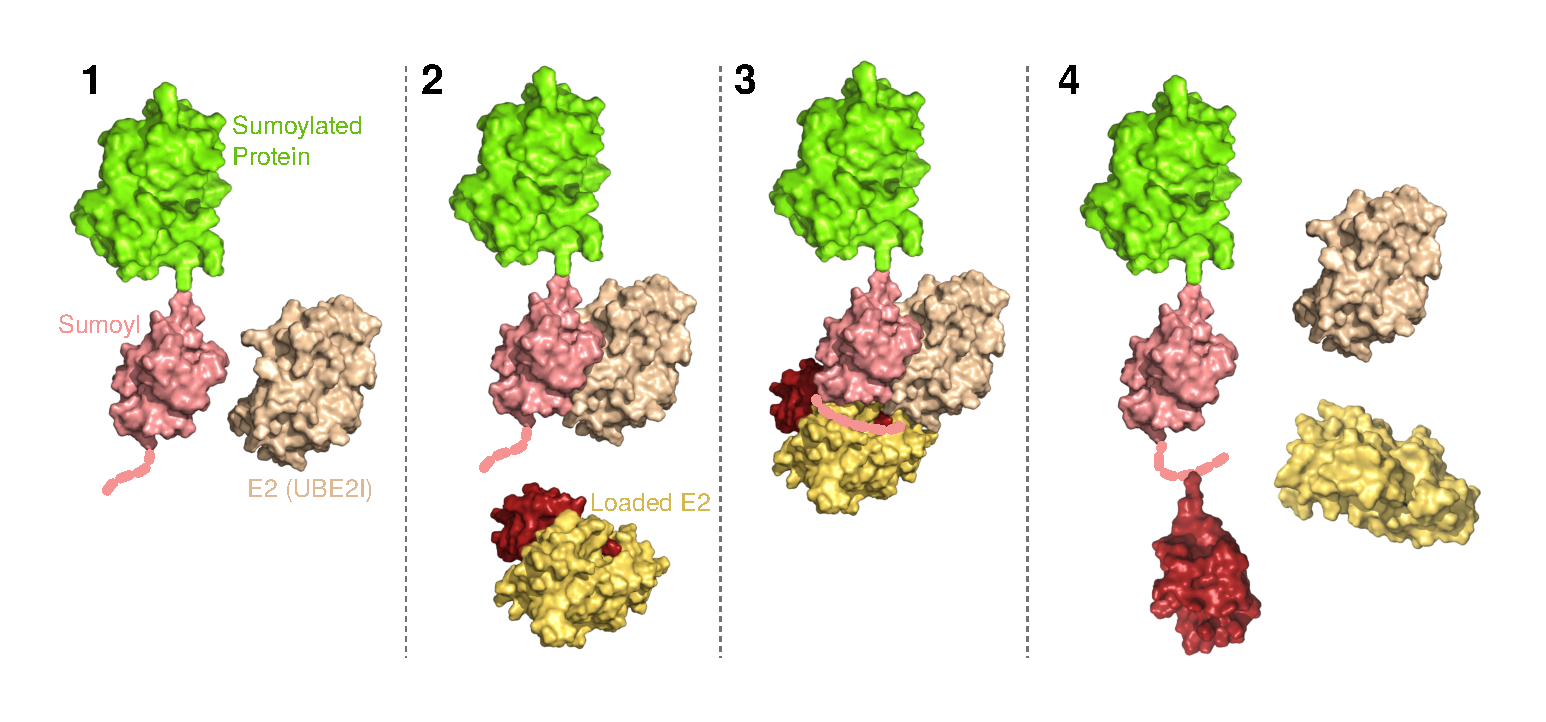
\includegraphics[width=\textwidth]{img/sumo_chaining.pdf}
	\caption{Steps in SUMO chain formation as proposed by Alontaga and colleagues~\cite{alontaga_rwd_2015}. An E2 noncovalently interacts with a SUMO modification of a target protein. A second E2 carrying a covalently bound second SUMO binds the first E2-SUMO complex, allowing for the first SUMO's N-terminal tail to enter the active site, where a lysine within the tail is forms a peptide bond with the second SUMO's C-terminus. Finally, the complex dissociates, leaving behind the newly formed SUMO chain. Images were generated using data from the following PDB structures: \texttt{3UIP}~\cite{gareau_determinants_2012}, \texttt{4Y1L}~\cite{alontaga_rwd_2015}}
	\label{fig:sumo_chaining}
\end{figure}

Like ubiquitin, SUMO can also form chains (Figure \ref{fig:sumo_chaining}). However, of the four SUMO proteins encoded by the human genome, only SUMO2 and SUMO3 are capable of doing so, as they contain a suitable lysine residue within a disordered N-terminal tail~\cite{tatham_polymeric_2001}. Capili and Lima previously observed that the E2 (UBE2I) and SUMO can interact in a noncovalent manner via a distinct binding interface~\cite{capili_structure_2007}. According to a model proposed by Alontaga and colleagues~\cite{alontaga_rwd_2015} this interaction is a key mechanism in SUMO chain formation. The interaction recruits a second, SUMO-loaded E2 that interacts with the complex in such a manner that the lysine within the first SUMO's N-terminal tail can find its way into the active site of the second E2, where the second SUMO is concatenated. While the role of polySUMO chains in humans are still unclear, it has been shown that yeast deficient in SUMO chain formation are unable to perform meiosis~\cite{cheng_sumo_2006}.

Given the complexity of the Sumoylation system, especially surrounding the E2 component, an examination of sequence-structure-function relationships becomes a multifaceted problem. Mutations could in principle affect any combination of the multiple interaction interfaces which in turn contribute in complex ways to the overall cellular phenotype.
An alanine scan of the yeast SUMO E2 Ubc9 was previously performed and succeeded in identifying functionally important sites within the protein~\cite{bencsath_identification_2002}. Similarly, a DMS scan of ubiquitin was previously completed~\cite{roscoe_analyses_2013}. While both of these projects provided great insight into the biochemistry of ubiquitin-like protein pathways, neither has produced a complete map. That is, not all possible amino acid changes were measured at high confidence levels. The Deep Mutational Scanning Framework we will discuss in chapter~\ref{ch:data1} enabled us to not only recapitulate many of the known mechansims in SUMO and its E2, but also to uncover new details about their biochemistry, as will be discussed in chapter~\ref{ch:data2}.